\documentclass[
11pt, fontset=Minion, toclevel=3, colorfullink=false,
linespread=1.414, lines=30, oneside, onesideheader,
mintcode, minted=cache,
draftnote, showoverfull
]{mthesis}
\let\firstyear\iftrue  \let\endfirstyear\fi
\let\secondyear\iftrue \let\endsecondyear\fi
\let\thirdyear\iffalse \let\endthirdyear\fi

\def\DeclareAbbr#1#2{\def#1{\textsc{#2}\xspace}}
\DeclareAbbr{\ess}{ess}
\DeclareAbbr{\aic}{aic}
\DeclareAbbr{\bic}{bic}
\DeclareAbbr{\dic}{dic}
\DeclareAbbr{\fic}{fic}
\DeclareAbbr{\fpe}{fpe}
\DeclareAbbr{\gic}{gic}
\DeclareAbbr{\mcmc}{mcmc}
\DeclareAbbr{\mdl}{mdl}
\DeclareAbbr{\mle}{mle}
\DeclareAbbr{\nic}{nic}
\DeclareAbbr{\nls}{nls}
\DeclareAbbr{\pet}{pet}
\DeclareAbbr{\rjmcmc}{rjmcmc}
\DeclareAbbr{\smc}{smc}
\DeclareAbbr{\tic}{tic}
\DeclareAbbr{\unix}{unix}

\def\bugs{\textsc{\sffamily bugs}\xspace}
\def\jags{\textsc{\sffamily jags}\xspace}

\def\aicc{\hbox{\aic{}\ensuremath{_c}}\xspace}

\def\kl{Kullback-Leibler divergence\xspace}
\def\mha{Metropolis-Hastings algorithm\xspace}

\def\dkl{D_{\mathrm{KL}}}

\def\bth{{\mathbfit{\theta}}}
\def\bTh{{\mathbfit{\Theta}}}

\def\hbth{\widehat{\bth}}
\def\tbth{\widetilde{\bth}}

\def\xm{(x^1,\dots,x^m)}
\def\Xm{(X^1,\dots,X^m)}
\def\bthm{(\bth^1,\dots,\bth^m)}
\def\bThm{(\bTh^1,\dots,\bTh^m)}
\def\vec#1#2{#1_1,\dots,#1_{#2}}
\def\svec#1#2{#1^1,\dots,#1^{#2}}
\def\mcvec#1#2{#1^{(1)},\dots,#1^{(#2)}}

\def\calGa{\mathcal{Ga}}
\def\calK{\mathcal{K}}
\def\calLN{\mathcal{LN}}
\def\calL{\mathcal{La}}
\def\calM{\mathcal{M}}
\def\calN{\mathcal{N}}

\def\bbN{\mathbb{N}}
\def\bbR{\mathbb{R}}

\def\bfX{\mathbfit{X}}
\def\bfx{\mathbfit{x}}
\def\bfY{\mathbfit{Y}}
\def\bfy{\mathbfit{y}}
\def\bfu{\mathbfit{u}}


\begin{document}
\begin{figure}[t]
  \linespread{1.1}\selectfont
  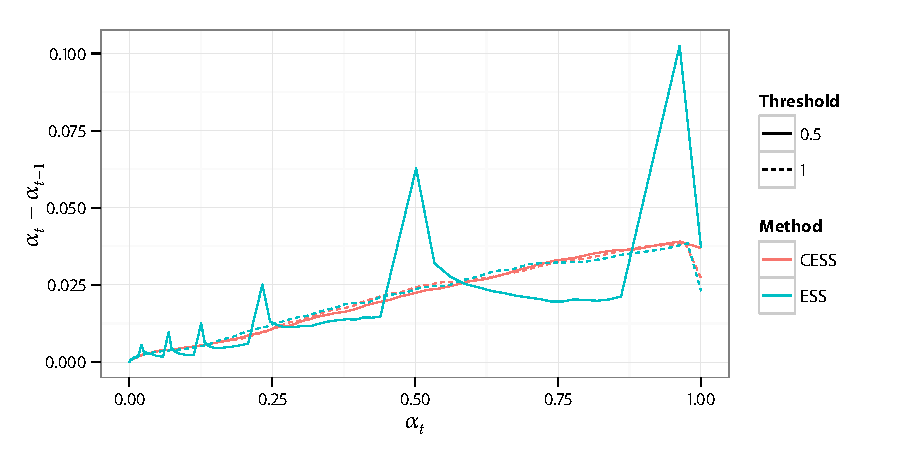
\includegraphics[width=\linewidth]{fig_src/Adaptive_Dist}
  \caption[Variations of the distribution specification parameter for the
  \protect\pet compartmental model using adaptive \protect\smc algorithms]
  {A typical plot of $\alpha_t - \alpha_{t-1}$ against $\alpha_t$ for the
    two-compartments \pet model with the simulated data set using the \smc[2]
    algorithm. The specifications of the adaptive parameter (\ess or \cess)
    are adjusted such that all four samplers use roughly the same number of
    distributions.}
  \label{fig:adaptive_alpha}
\end{figure}
     \clearpage
\begin{figure}[t]
  \linespread{1.1}\selectfont
  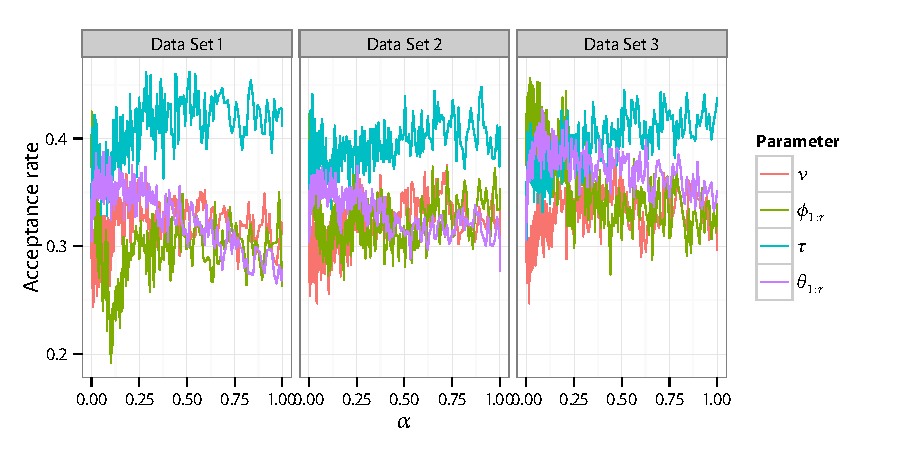
\includegraphics[width=\linewidth]{fig_src/Adaptive_Proposal}
  \caption[Acceptance rates of adaptive \protect\smc algorithms]
  {Average random walk acceptance rates for the two-compartments \pet model
    with data sets in Figure~\ref{fig:typical real pet} using adaptive
    proposal scales}
  \label{fig:pet adaptive proposal}
\end{figure}
 \clearpage
\begin{figure}[t]
  \linespread{1.1}\selectfont
  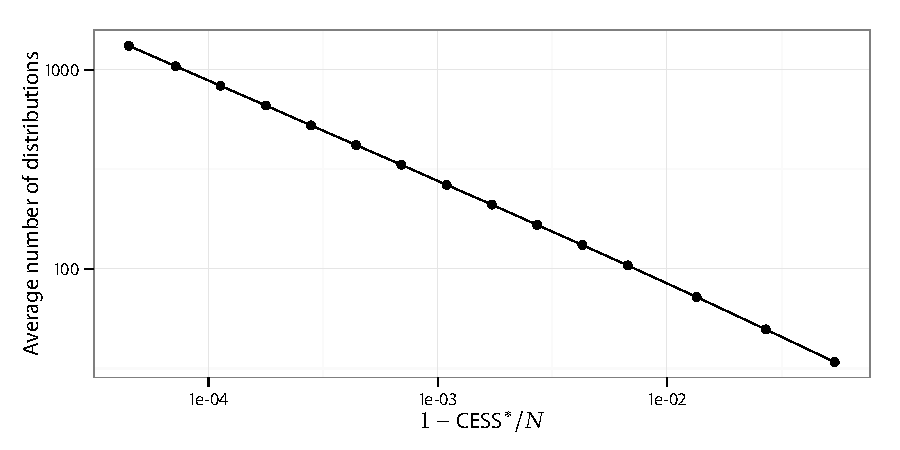
\includegraphics[width=\linewidth]{fig_src/CESS_Iter_Mean}
  \caption[Relations between average number of distributions and
  \protect\cess]
  {Relations between average number of distributions and $\cess^\star$ for the
    two-compartments \pet model with the simulated data set using the \smc[2]
    algorithm. The number of distributions ranges from $\sim$30 to
    $\sim$1,300.}
  \label{fig:cess iter mean}
\end{figure}
    \clearpage
\begin{figure}[t]
  \UseAltLinespread
  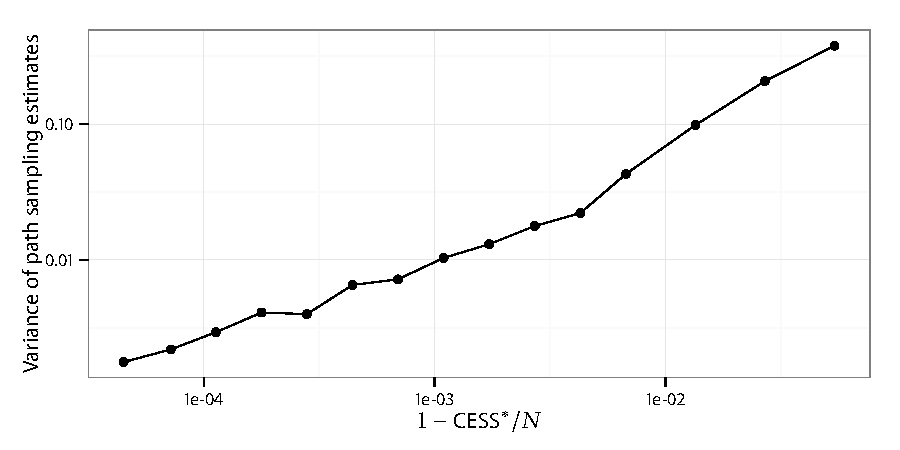
\includegraphics[width=\linewidth]{fig_src/CESS_Path_Var}
  \caption[Relations between the variance of the path sampling estimator and
  \protect\cess]
  {Relationship between the variance of the path sampling estimator and $\cess^\star$ for the two-compartments \pet model with the simulated data set using the \smc[2] algorithm (on logarithm scale). The variances are calculated from 100 simulations for each sampler configuration.}
  \label{fig:cess path var}
\end{figure}
     \clearpage
\begin{figure}[t]
  \UseAltLinespread
  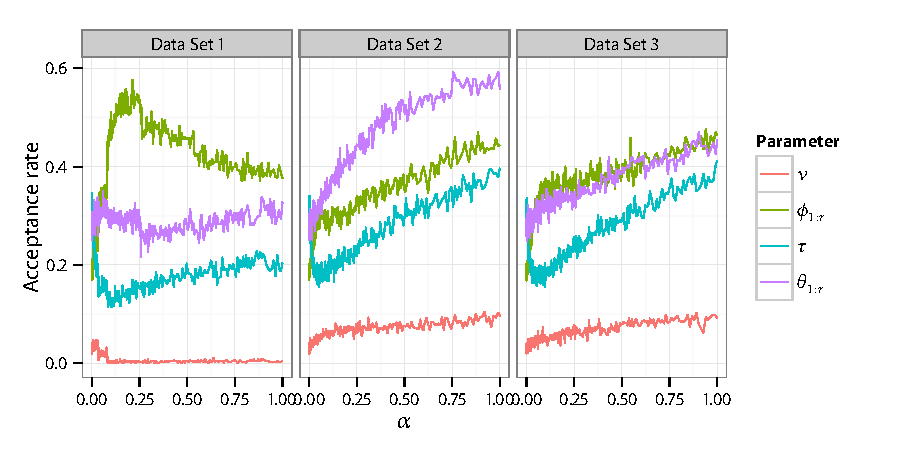
\includegraphics[width=\linewidth]{fig_src/Fixed_Proposal}
  \caption[Acceptance rates of non-adaptive \protect\smc algorithms]
  {Average random walk acceptance rates for the two-compartments \pet model
    with data sets in Figure~\ref{fig:typical real pet} using fixed proposal
    scales.}
  \label{fig:pet fixed proposal}
\end{figure}
    \clearpage
\begin{figure}[t]
  \linespread{1.1}\selectfont
  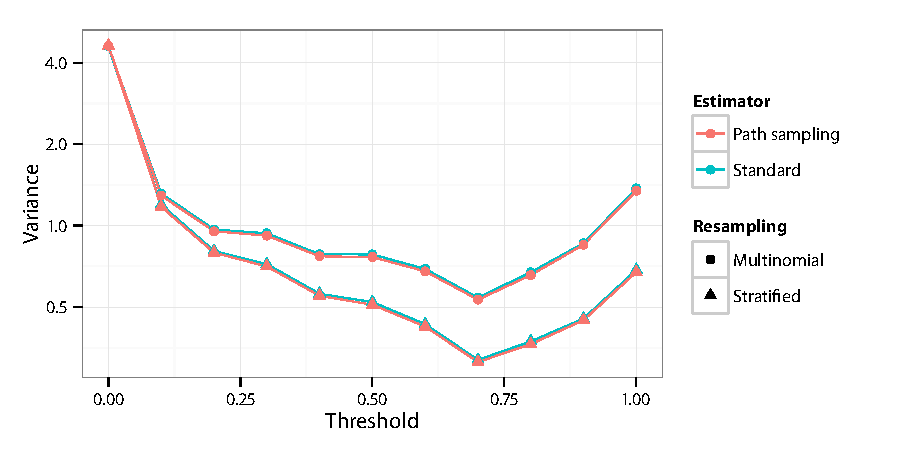
\includegraphics[width=\linewidth]{fig_src/GMM_Resample}
  \caption[Variance of standard standard estimator and path sampling using
  adaptive resampling]
  {Monte Carlo variance of standard estimator and path sampling estimator
    using different threshold of $\ess/N$ for Gaussian mixture model using the
    \smc[2] algorithm and the stratified resampling. The variances are plotted
    on log scale.}
  \label{fig:gmm resample}
\end{figure}
      \clearpage
\begin{figure}[t]
  \linespread{1.1}\selectfont
  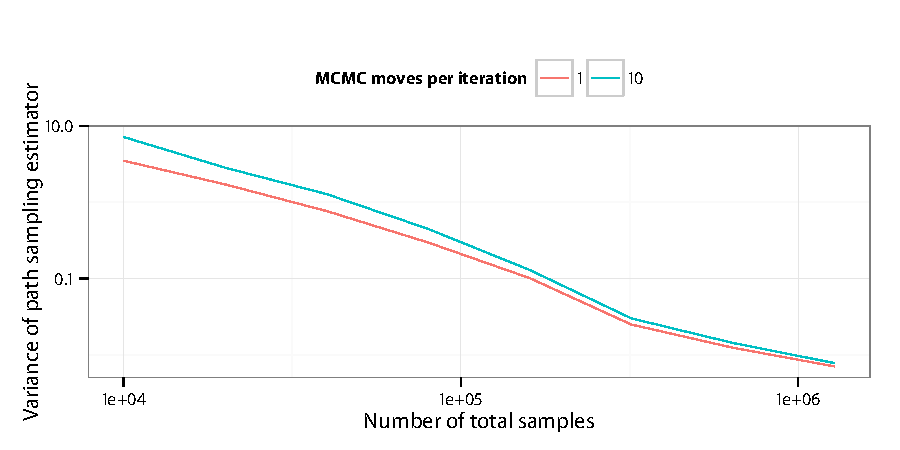
\includegraphics[width=\linewidth]{fig_src/MCMC_Iter_Var}
  \caption[Variance of path sampling estimator and total number of samples
  using \protect\smc algorithm]
  {Variance of the path sampling estimates and total number of samples
    using the \smc[2] algorithm. Both samplers use 1,000 particles but with
    different number of distributions and passes of \mcmc moves at each
    iteration}
  \label{fig:fast mcmc iter}
\end{figure}
     \clearpage
\begin{figure}[t]
  \UseAltLinespread
  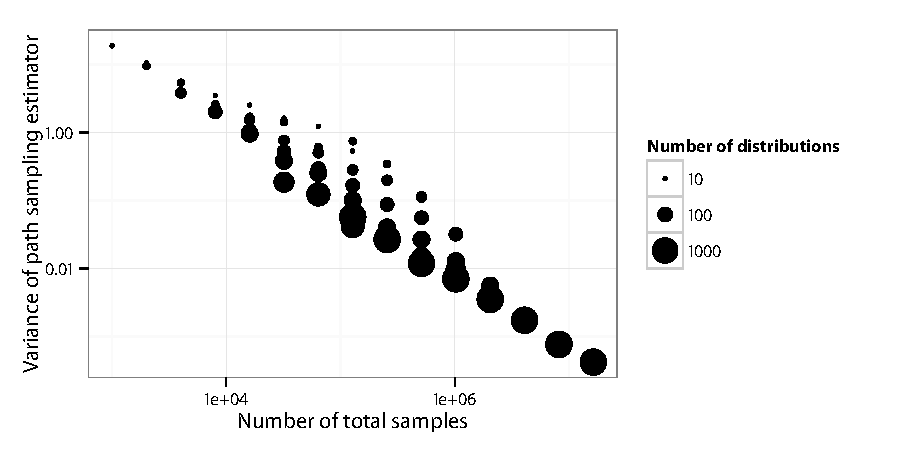
\includegraphics[width=\linewidth]{fig_src/Particle_Iter_Var}
  \caption[Variance of path sampling estimator and total number of samples
  using \protect\smc algorithm]
  {Variance of path sampling estimator and total number of samples using the
    \smc[2] algorithm. Multiple samplers are used to evluate the trade-off
    between the number of particles $N$ and the number of distributions $T$.
    They are configured such that the total number of samples $NT$ is a
    constant. In this figure, the variance of the path sampling estimator from
    100 simulations of each sampler is plotted against the total number of
    samples $NT$ on the log scale. Different configurations of $T$ are
    indicated with different sizes of the dots, larger dots representing
    larger $T$ (and thus smaller $N$). It can be seen that for a particular
    value of $NT$, changing $T$ may change the variance considerably and
    larger $T$ is preferred for most values of $NT$.}
  \label{fig:particle iter num}
\end{figure}
 \clearpage
\begin{figure}[t]
  \linespread{1.1}\selectfont
  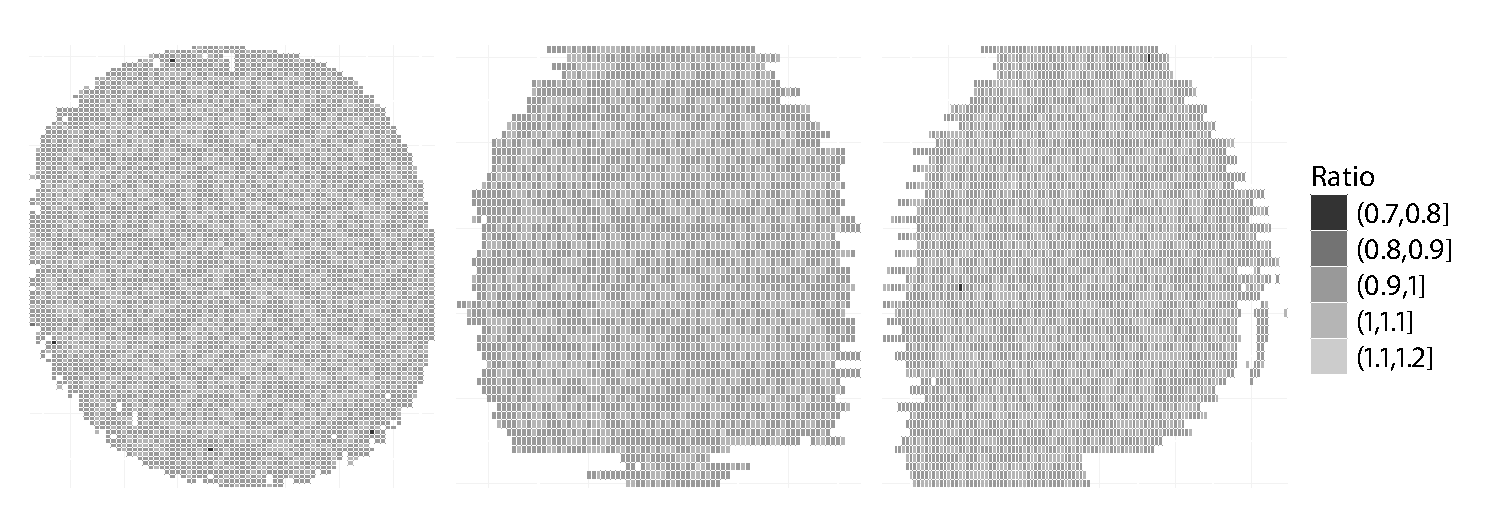
\includegraphics[width=\linewidth]{fig_src/PET_Converge}
  \caption[Convergence diagnostics for the random walk algorithm for the
  \protect\pet compartmental model using summary statistics]
  {Convergence diagnostics for the three-compartments \pet using ratio of
    variance of $V_D$ estimates using final 1,000 samples to that of all
    10,000 post burn-in samples.}
  \label{fig:pet diag ratio}
\end{figure}
      \clearpage
\begin{figure}[t]
  \UseAltLinespread
  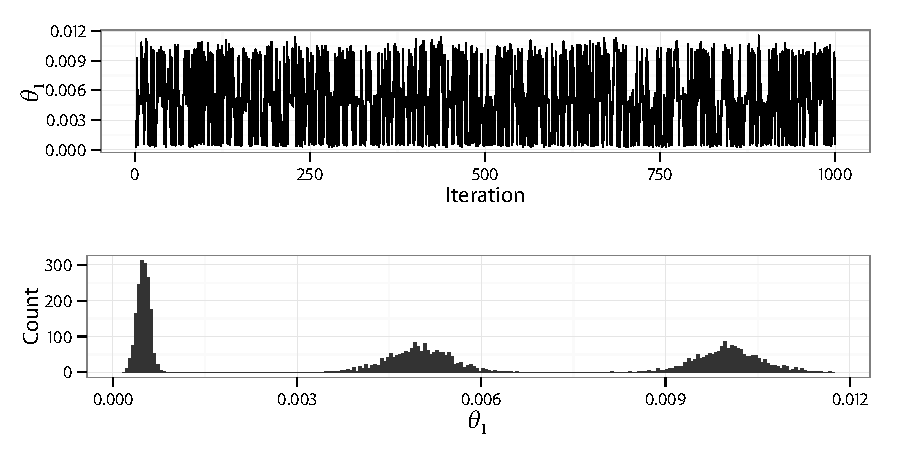
\includegraphics[width=\linewidth]{fig_src/PET_MH_Diag_C}
  \caption[Trace and histogram of parameters in the random walk algorithm for
  the \protect\pet compartmental model (uncalibrated)]
  {Trace and histogram plots of parameter $\theta_1$ from a \mcmc
    sampler for \pet model with three components and non-informative priors
    without ordering. The trace plot has 1,000 samples and the histogram plot
    has 10,000 samples. The sampler is well calibrated.}
  \label{fig:pet diag c}
\end{figure}
     \clearpage
\begin{figure}[t]
  \linespread{1.1}\selectfont
  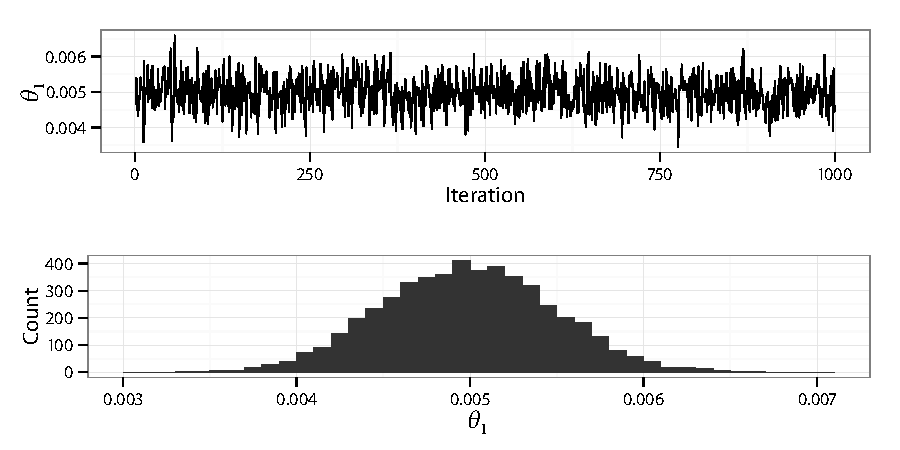
\includegraphics[width=\linewidth]{fig_src/PET_MH_Diag}
  \caption[Trace and histogram of parameters in the random walk algorithm for
  the \protect\pet compartmental model (calibrated)]
  {Trace and histogram plots of parameter $\theta_1$ from a \mcmc
    sampler for \pet model with three components and non-informative priors
    without ordering. The trace plot has 1,000 samples and the histogram plot
    has 10,000 samples. The sampler is not well calibrated.}
  \label{fig:pet diag}
\end{figure}
       \clearpage
\begin{figure}[t]
  \UseAltLinespread
  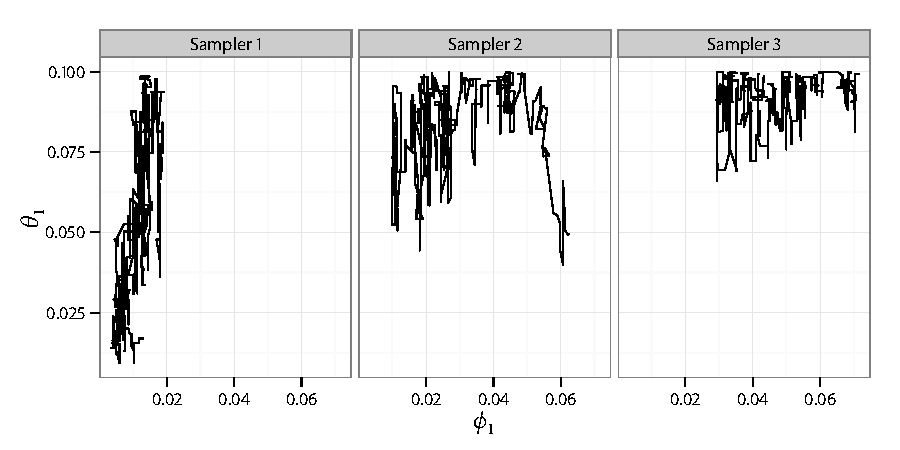
\includegraphics[width=\linewidth]{fig_src/PET_MH_H_Path.pdf}
  \caption[Traces of parameters in the random walk algorithm for the
  \protect\pet compartmental model (uncalibrated)]
  {Trace of $(\phi_1,\theta_1)$ from three random walk Metropolis-Hastings samplers for the one-compartments \pet model with non-informative priors, using proposal scales five times of those tuned.}
  \label{fig:pet mh untuned}
\end{figure}
     \clearpage
\begin{figure}
  \linespread{1.1}\selectfont
  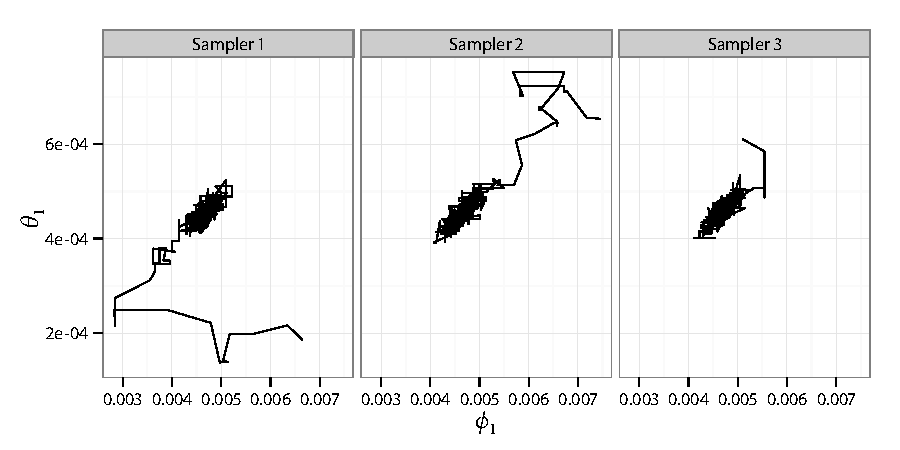
\includegraphics[width=\linewidth]{fig_src/PET_MH_Path.pdf}
  \caption[Traces of parameters in the random walk algorithm for the
  \protect\pet compartmental model (calibrated)]
  {Trace of $(\phi_1,\theta_1)$ from three random walk Metropolis-Hastings
  samplers for the one-compartments \pet model with non-informative priors,
  using well tuned proposal scales. The first few values of each trace is not
  shown in the plots since they are far away from the high probability region
  with an order of magnitude difference in values.}
  \label{fig:pet mh tuned}
\end{figure}
       \clearpage
\begin{figure}[t]
  \UseAltLinespread
  \centering
  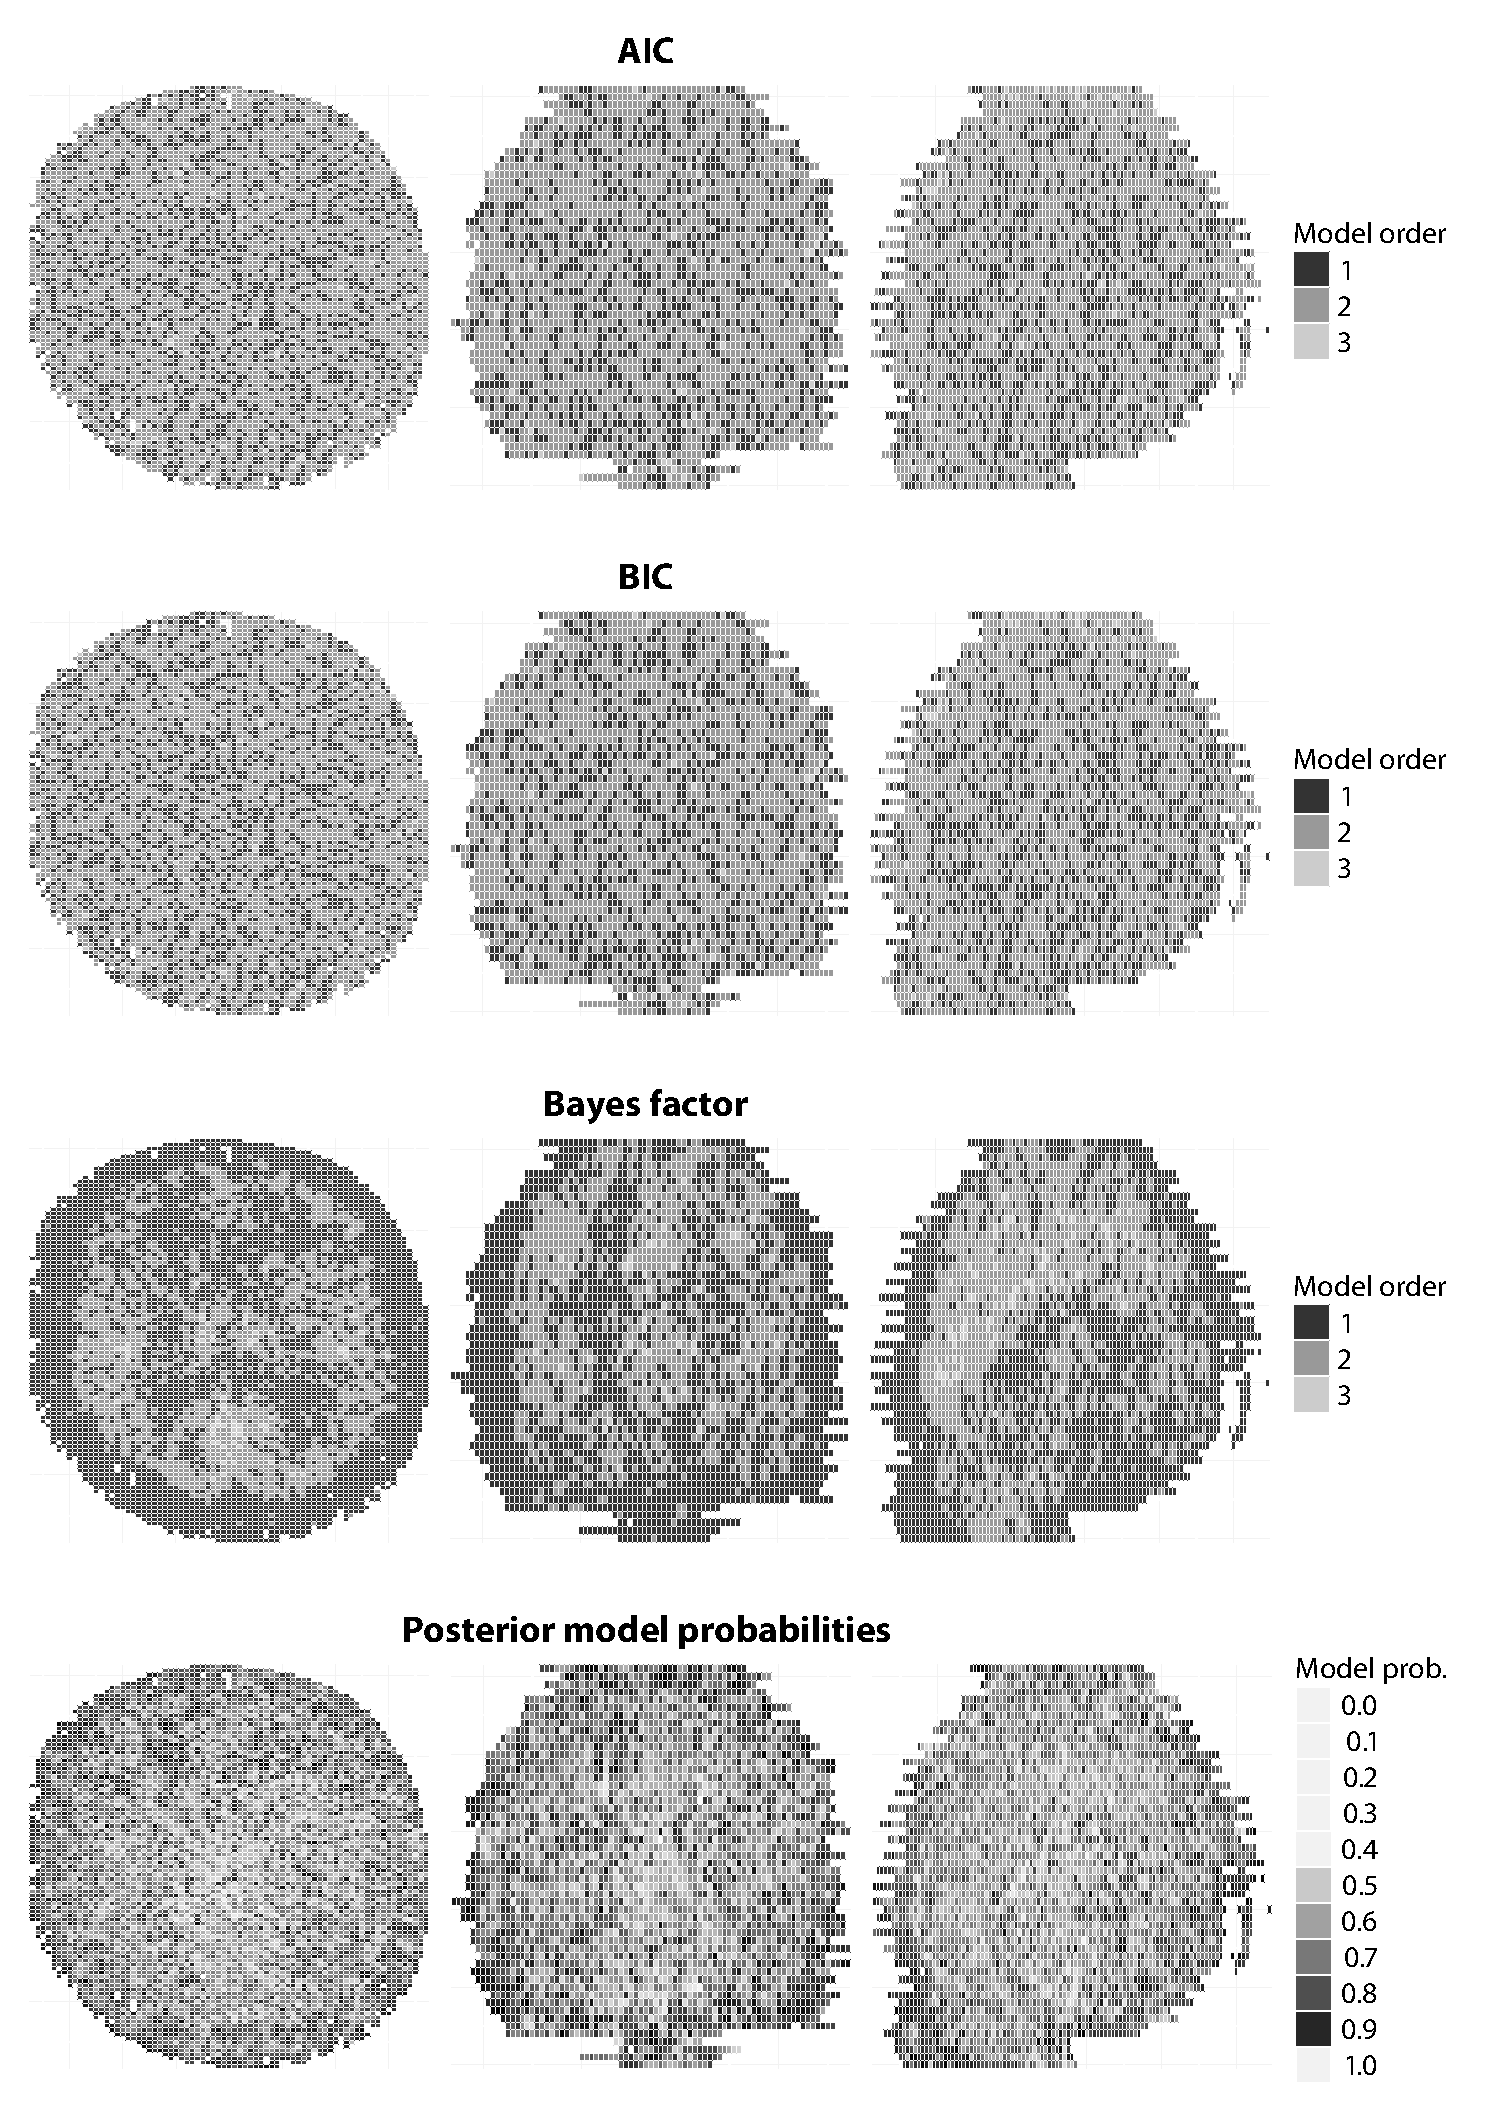
\includegraphics[width=0.95\linewidth]{fig_src/PET_MO}
  \caption[Model selection results for the \protect\pet compartmental model]
  {Model selection results for \pet model using real data set. From
    top to bottom: Model order selected by \aicc (see Section~\ref{sub:A
      second order aic}); Model order selected by \bic (see
    Section~\ref{sub:Bayes factor}); Model order selected by using Bayesian
    model comparison with marginal likelihood approximated by generalized
    harmonic mean estimator; The posterior model probability
    $\pi(\calM_k|\data)$ (see Section~\ref{sub:Model choice problems}) with
    uniform prior model probability $\pi(\calM_k)$.}
  \label{fig:pet mo}
\end{figure}
            \clearpage
\begin{figure}[t]
  \UseAltLinespread
  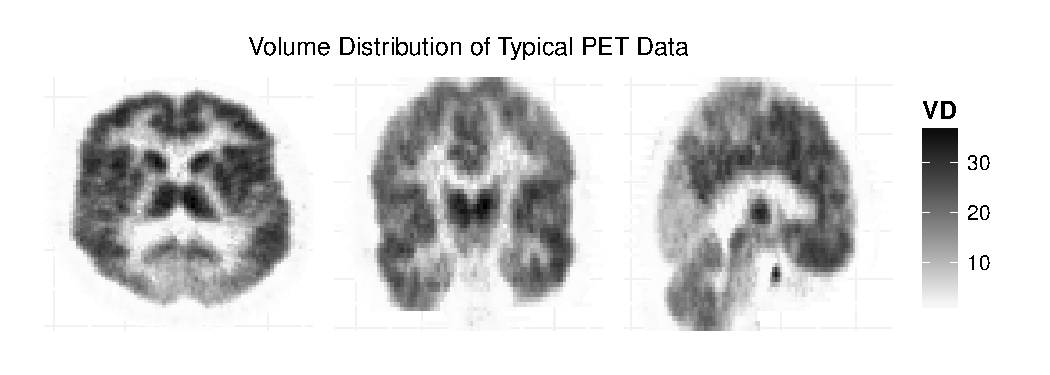
\includegraphics[width=\linewidth]{fig_src/PETPlot-smc2-ps-bw}
  \caption[Volume of distribution of real \protect\pet compartmental model
  data]
  {Estimates of $V_D$ from a single \pet scan as found using \smc[2].
    The data shows that the volume of distribution exhibits substantial
    spatial variation. Note that each pixel in the image represent an estimate
    from an individual time series data set. There are approximately a quarter
    of a million of them and each requires a Monte Carlo simulation to select
    a model.}
  \label{fig:petplot}
\end{figure}
          \clearpage
\begin{figure}[t]
  \UseAltLinespread
  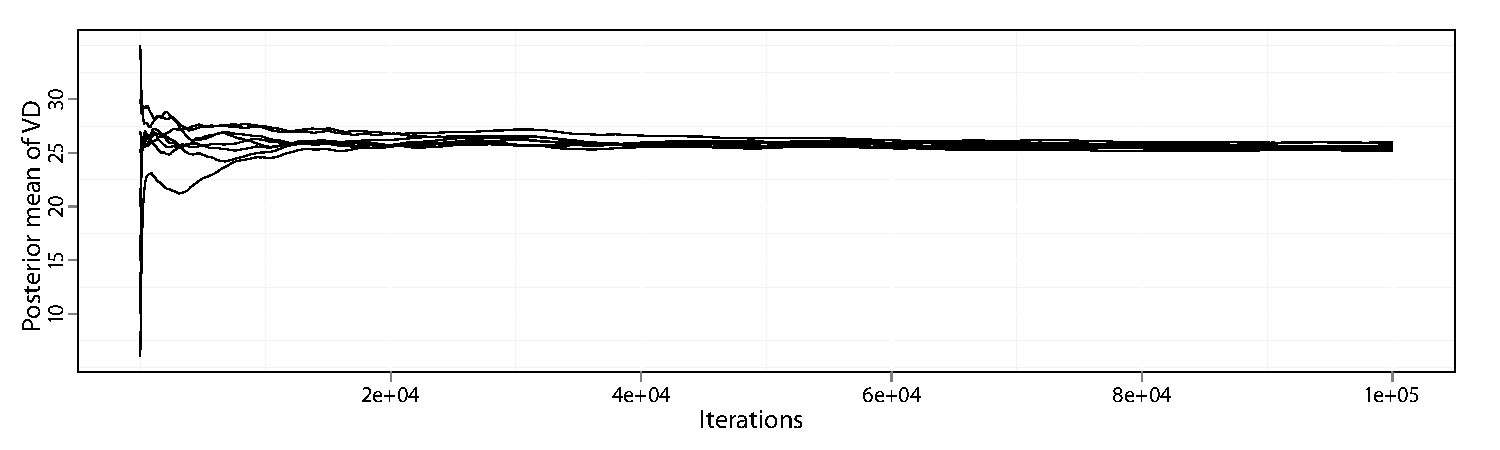
\includegraphics[width=\linewidth]{fig_src/PET_VD}
  \caption[Convergence diagnostics for the random walk algorithm for the
  \protect\pet compartmental model using averages]
  {Estimates of $V_D$ when starting the \mcmc chain from different
    values for a typical data set of a \pet model with three component.}
  \label{fig:pet vd mean}
\end{figure}
            \clearpage
\begin{figure}[t]
  \UseAltLinespread
  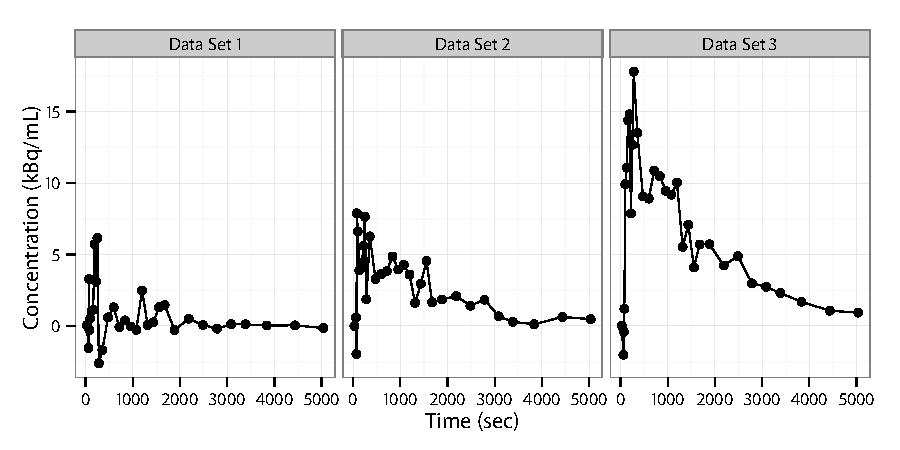
\includegraphics[width=\linewidth]{fig_src/Typical_PET}
  \caption
  [Typical real \protect\pet data]
  {Typical real \protect\pet data.}
  \label{fig:typical real pet}
\end{figure}
       \clearpage
\begin{figure}
  \linespread{1.1}\selectfont
  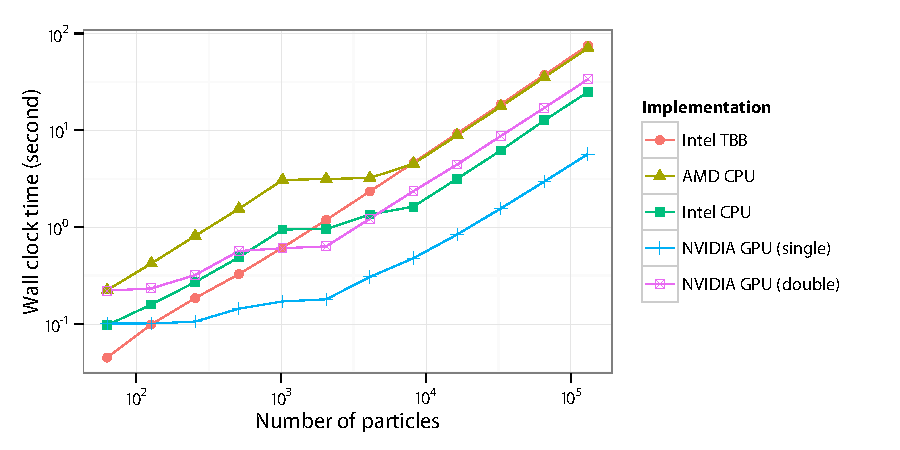
\includegraphics[width=\linewidth]{fig_src/bench-ocl-time-running}
  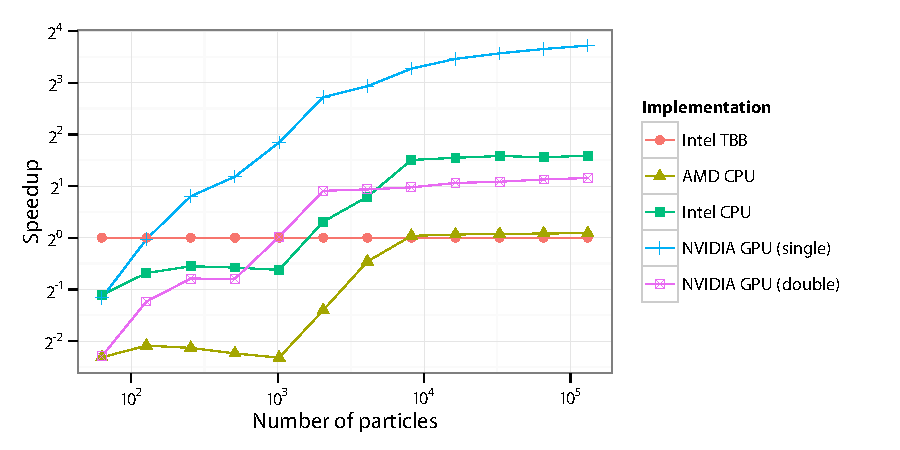
\includegraphics[width=\linewidth]{fig_src/bench-ocl-speedup-running}
  \caption[Performance of \protect\vsmc \protect\opencl implementations]
  {Performance of \opencl implementations of Bayesian modeling for
    Gaussian mixture model (Linux; Xeon W3550 \gpu, 3.06GHz, 4 cores, 8
    threads; NVIDIA Quadro 2000).}
  \label{fig:bench-ocl-perf}
\end{figure}
    \clearpage
\begin{figure}
  \UseAltLinespread
  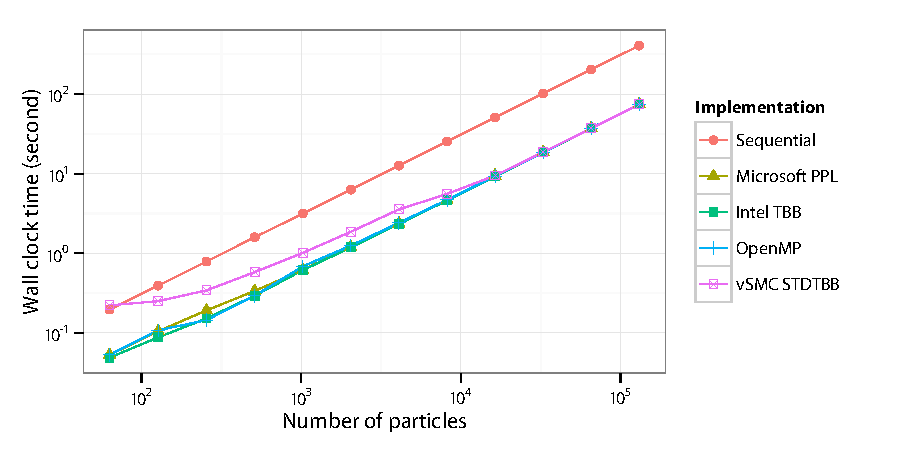
\includegraphics[width=\linewidth]{fig_src/bench-smp-time-running}
  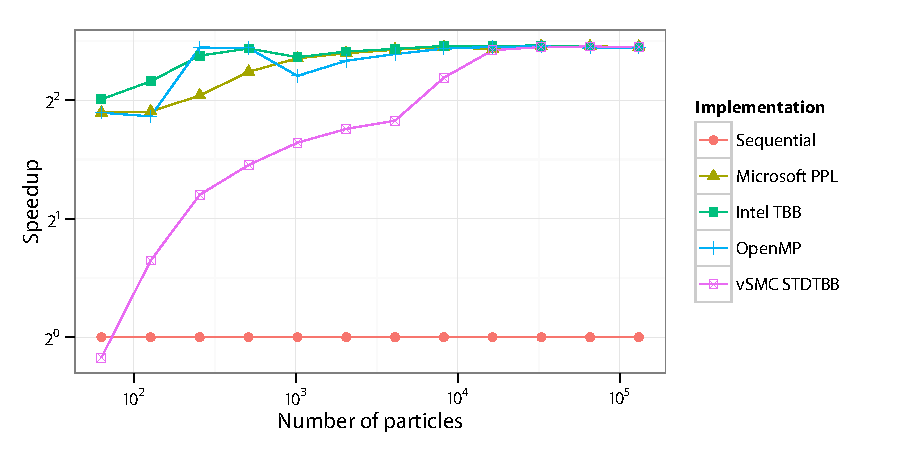
\includegraphics[width=\linewidth]{fig_src/bench-smp-speedup-running}
  \caption[Performance of \protect\vsmc \protect\smp implementations]
  {Performance of \cpp implementations of Bayesian modeling for Gaussian mixture model (Linux; Xeon W3550, 3.06GHz, 4 cores, 8 threads). The top plots the wall clock time against the number of particles. The bottom plots the the speedup relative the sequential implementation against the number of particles.}
  \label{fig:bench-smp-perf}
\end{figure}
    \clearpage
\end{document}
